\documentclass[svgnames,11pt]{beamer}
\input{/home/tof/Documents/Cozy/latex-include/preambule_commun.tex}
\input{/home/tof/Documents/Cozy/latex-include/preambule_beamer.tex}
%\usepackage{pgfpages} \setbeameroption{show notes on second screen=left}
\author[]{Christophe Viroulaud}
\title{Construire une image numérique\\Introduction à Python}
\date{\framebox{\textbf{Phot 02}}}
%\logo{}
\institute{Seconde - SNT}

\begin{document}
\begin{frame}
\titlepage
\end{frame}
\begin{frame}
    \frametitle{}
Une image numérique est composée de points colorés appelés \textbf{pixels}.
   \begin{center}
       \begin{tabular}{cc}
           \includegraphics[width=4cm,height=3cm]{ressources/vigne.jpg}
           &
           \includegraphics[width=4cm,height=3cm]{ressources/vigne-pixel.png}
       \end{tabular}
   \end{center} 
Pour construire une image numérique il suffit d'aligner suffisamment de points.
\end{frame}
\begin{frame}
    \frametitle{}

    \begin{framed}\centering 
        Comment construire une image numérique par programmation?
    \end{framed}

\end{frame}
\section{Stocker une image en mémoire}
\begin{frame}[fragile]
    \frametitle{Stocker une image en mémoire}

Pour pouvoir utiliser des données dans un programme, il faut les stocker dans une variable.
\begin{center}
    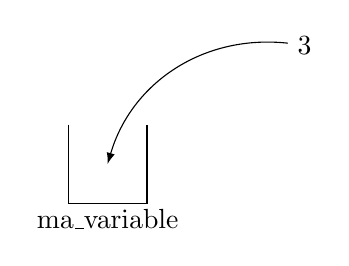
\begin{tikzpicture}
        \draw (0,1) -- (0,0) -- (1,0) -- (1,1);
        \node (3) at (3,2) {3};
        \node at (.5,-.2) {ma\_variable};
        \draw[->,>=latex] (3) to[bend right=40] (.5,.5);

    \end{tikzpicture}
    \captionof{figure}{Affectation}
\end{center}

\begin{center}
    \begin{lstlisting}[language=Python , basicstyle=\ttfamily\small, xleftmargin=2em, xrightmargin=2em]
ma_variable = 3
\end{lstlisting}
    \captionof{code}{Créer une variable en Python}
    \label{CODE}
    \end{center}
\end{frame}
\begin{frame}[fragile]
    \frametitle{}
\begin{center}
\begin{lstlisting}[language=Python , basicstyle=\ttfamily\small, xleftmargin=0em, xrightmargin=0em]
# Créer une variable 'image'
image = Image.new('RGB', (800, 600), (255, 255, 255))
\end{lstlisting}
\captionof{code}{Stocker une image blanche}
\label{CODE}
\end{center}

\begin{center}
    \begin{tikzpicture}
        \draw (0,1) -- (0,0) -- (1,0) -- (1,1);
        \node at (.5,-.2) {image};
        \draw (2,2) -- (4,2) -- (4,3) -- (2,3) -- cycle;
        \draw[->,>=latex] (3,2.5) to[bend right=40] (.5,.5);

    \end{tikzpicture}
    \captionof{figure}{Affecter une image vide dans \textbf{\texttt{image}}}
\end{center}

\end{frame}
\begin{frame}[fragile]
    \frametitle{}
\begin{activite}
\begin{enumerate}
    \item Ouvrir le logiciel \emph{Spyder}.
    \item Écrire le code \ref{image} dans la partie gauche.
    \item Enregistrer le programme dans le dossier \textbf{SNT} sous le nom \textbf{\texttt{mon\_image.py}}
\end{enumerate}
\end{activite}
\begin{center}
\begin{lstlisting}[language=Python , basicstyle=\ttfamily\small, xleftmargin=0.em, xrightmargin=0.em]
# Bibliothèque de gestion des images
from PIL import Image
# Créer une variable 'image'
image = Image.new('RGB', (800, 600), (255, 255, 255))
# Afficher l'image
image.show()
\end{lstlisting}
\captionof{code}{Afficher l'image}
\label{image}
\end{center}

\end{frame}
\section{Répéter une opération}
\begin{frame}[fragile]
    \frametitle{Répéter une opération}

Pour modifier l'image blanche, il faut poser des pixels d'une autre couleur.
\begin{center}
    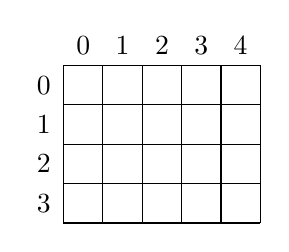
\begin{tikzpicture}[scale=0.5]
    \draw (0,0) grid (5,4);
    
    \draw (-0.5,3.5) node{0};
    \draw (-0.5,2.5) node{1};
    \draw (-0.5,1.5) node{2};
    \draw (-0.5,0.5) node{3};
    \draw (0.5,4.5) node{0};
    \draw (1.5,4.5) node{1};
    \draw (2.5,4.5) node{2};
    \draw (3.5,4.5) node{3};
    \draw (4.5,4.5) node{4};
    \end{tikzpicture}
    \captionof{figure}{Coordonnées d'un pixel}
\begin{lstlisting}[language=Python , basicstyle=\ttfamily\small, xleftmargin=0em, xrightmargin=0em]
from PIL import Image
image = Image.new('RGB', (800, 600), (255, 255, 255))
# Poser un pixel noir en (10,10)
image.putpixel((10,10),(0,0,0))
image.show()
\end{lstlisting}
\captionof{code}{Poser un pixel}
\label{CODE}
\end{center}
\end{frame}
\begin{frame}
    \frametitle{}

    \begin{activite}
    Poser plusieurs pixels noirs à côté du premier jusqu'à voir une forme sur l'image.
    \end{activite}

\end{frame}
\begin{frame}[fragile]
    \frametitle{Correction}
\begin{center}
\begin{lstlisting}[language=Python , basicstyle=\ttfamily\small, xleftmargin=2em, xrightmargin=2em]
image.putpixel((10,10),(0,0,0))
image.putpixel((11,10),(0,0,0))
image.putpixel((12,10),(0,0,0))
image.putpixel((13,10),(0,0,0))
image.putpixel((11,10),(0,0,0))
image.putpixel((11,11),(0,0,0))
image.putpixel((11,12),(0,0,0))
image.putpixel((11,13),(0,0,0))
image.putpixel((12,10),(0,0,0))
image.putpixel((12,11),(0,0,0))
image.putpixel((12,12),(0,0,0))
image.putpixel((12,13),(0,0,0))
\end{lstlisting}
\captionof{code}{}
\label{CODE}
\end{center} 

\end{frame}
\begin{frame}[fragile]
    \frametitle{}

\begin{center}
\begin{lstlisting}[language=Python , basicstyle=\ttfamily\small, xleftmargin=2em, xrightmargin=2em]
for x in range(100):
    image.putpixel((x,10),(0,0,0))
\end{lstlisting}
\captionof{code}{Répéter une opération}
\label{CODE}
\end{center}

\end{frame}
\begin{frame}[fragile]
    \frametitle{}

    \begin{activite}
    \begin{enumerate}
        \item Remplacer les ajouts manuels de pixels par le code \ref{repete}.
\begin{center}
\begin{lstlisting}[language=Python , basicstyle=\ttfamily\small, xleftmargin=2em, xrightmargin=2em]
for x in range(100):
    image.putpixel((x,10),(0,0,0))
\end{lstlisting}
\captionof{code}{Répéter une opération}
\label{repete}
\end{center}
\item Modifier le code pour tracer un trait sur toute la largeur de l'image.
        \item Créer une nouvelle boucle pour tracer un trait vertical.
        \item Tracer un trait oblique.
    \end{enumerate}
    \end{activite}

\end{frame}
\begin{frame}[fragile]
    \frametitle{Correction}

\begin{center}
\begin{lstlisting}[language=Python , basicstyle=\ttfamily\small, xleftmargin=2em, xrightmargin=2em]
# horizontal
for x in range(800):
    image.putpixel((x,10),(0,0,0))

# vertical
for y in range(600):
    image.putpixel((400,y),(0,0,0))

# oblique
for y in range(600):
    image.putpixel((y,y),(0,0,0))
\end{lstlisting}
\captionof{code}{Tracé de trois traits}
\label{CODE}
\end{center}

\end{frame}
\section{Fonction}
\begin{frame}[fragile]
    \frametitle{Fonction}

\begin{center}
\begin{lstlisting}[language=Python , basicstyle=\ttfamily\small, xleftmargin=2em, xrightmargin=2em]
for x in range(800):
    image.putpixel((x,10),(0,0,0))

for x in range(800):
    image.putpixel((x,20),(0,0,0))

for x in range(800):
    image.putpixel((x,30),(0,0,0))

for x in range(800):
    image.putpixel((x,40),(0,0,0))
\end{lstlisting}
\captionof{code}{Répétition de code}
\label{CODE}
\end{center}

\end{frame}
\begin{frame}
    \frametitle{}
Pour éviter de répéter du code on peut utiliser une \textbf{fonction}.
\begin{center}
    \begin{tabular}{ccc}
\includegraphics[width=3cm]{ressources/marteau1.jpg}
&
\includegraphics[width=3cm]{ressources/marteau2.jpg}
&
\includegraphics[width=3cm]{ressources/marteau3.jpg}
\\
marteau(petit)&marteau(moyen)&marteau(gros)\\
    \end{tabular}
\end{center}
\begin{aretenir}[]
Une fonction est un outil qui possède des \textbf{paramètres} et que l'on peut réutiliser dans le programme.
\end{aretenir}
\end{frame}
\begin{frame}[fragile]
    \frametitle{}

\begin{center}
\begin{lstlisting}[language=Python , basicstyle=\ttfamily\small, xleftmargin=2em, xrightmargin=2em]
def trait_horizontal(image, position):
    for x in range(800):
        image.putpixel((x,position),(0,0,0))
\end{lstlisting}
\captionof{code}{Construction de la fonction}
\label{CODE}
\end{center}

\begin{center}
\begin{lstlisting}[language=Python , basicstyle=\ttfamily\small, xleftmargin=2em, xrightmargin=2em]
trait_horizontal(image, 10)
\end{lstlisting}
\captionof{code}{Appel de la fonction}
\label{CODE}
\end{center}

\end{frame}
\begin{frame}[fragile]
    \frametitle{}

\begin{center}
\begin{lstlisting}[language=Python , basicstyle=\ttfamily\small, xleftmargin=0.em, xrightmargin=0.em]
from PIL import Image

def trait_horizontal(image, position):
    for x in range(800):
        image.putpixel((x,position),(0,0,0))

image = Image.new('RGB', (800, 600), (255, 255, 255))

trait_horizontal(image, 10)

image.show()
\end{lstlisting}
\captionof{code}{Afficher l'image}
\label{img}
\end{center} 
\begin{aretenir}[]
    On crée la fonction en début de programme puis on l'utilise quand on le souhaite.
    \end{aretenir}
\end{frame}
\begin{frame}[fragile]
    \frametitle{}

    \begin{activite}
    \begin{enumerate}
        \item Écrire la fonction \textbf{\texttt{trait\_vertical(image, position)}} qui trace un trait vertical.
        \item Dans le programme principal, écrire le code \ref{horiz}.
\begin{center}
\begin{lstlisting}[language=Python , basicstyle=\ttfamily\small, xleftmargin=2em, xrightmargin=2em]
for y in range(0,600,10):
    trait_horizontal(image, y)
\end{lstlisting}
\captionof{code}{}
\label{horiz}
\end{center}
\item En s'appuyant sur le code \ref{horiz}, tracer des lignes verticales tous les 10 pixels.
    \end{enumerate}
    \end{activite}

\end{frame}
\begin{frame}[fragile]
    \frametitle{Correction}

\begin{center}
\begin{lstlisting}[language=Python , basicstyle=\ttfamily\small, xleftmargin=2em, xrightmargin=2em]
def trait_vertical(image, position):
    for y in range(600):
        image.putpixel((position,y),(0,0,0))
\end{lstlisting}
\captionof{code}{Fonction pour un trait vertical}
\end{center}
\begin{center}
\begin{lstlisting}[language=Python , basicstyle=\ttfamily\small, xleftmargin=2em, xrightmargin=2em]
for x in range(0,800,10):
    trait_vertical(image, x)
\end{lstlisting}
\captionof{code}{Traits verticaux}
\end{center}

\end{frame}

\begin{frame}
    \frametitle{}

    \begin{activite}
    \begin{enumerate}
        \item Modifier la fonction \textbf{\texttt{trait\_horizontal(image, position, couleur)}} pour qu'elle trace un trait de la couleur désirée.
        \item Écrire la fonction \textbf{\texttt{carre(image, o\_x, o\_y, longueur)}} qui trace un carré dont le sommet haut gauche est en \texttt{\textbf{(o\_x, o\_y)}} et de côté \textbf{\texttt{longueur}}.
    \end{enumerate}
    \end{activite}

\end{frame}
\begin{frame}[fragile]
    \frametitle{Correction}
\begin{center}
\begin{lstlisting}[language=Python , basicstyle=\ttfamily\small, xleftmargin=1em, xrightmargin=1.5em]
def trait_horizontal(image, position, couleur):
    for x in range(800):
        image.putpixel((x, position), couleur)
\end{lstlisting}
\captionof{code}{Trait de couleur}
\label{CODE}
\end{center}

\begin{center}
\begin{lstlisting}[language=Python , basicstyle=\ttfamily\small, xleftmargin=2em, xrightmargin=1.5em]
trait_horizontal(image, 100, (120, 200, 150))
\end{lstlisting}
\captionof{code}{Appel de la fonction dans le programme}
\label{CODE}
\end{center}

\end{frame}
\begin{frame}[fragile]
    \frametitle{Correction}
\begin{center}
\begin{lstlisting}[language=Python , basicstyle=\ttfamily\small, xleftmargin=2em, xrightmargin=2em]
def carre(image, o_x, o_y, longueur):
    for x in range(o_x, o_x+longueur):
        for y in range(o_y, o_y+longueur):
            image.putpixel((x, y), (0, 0, 0))
\end{lstlisting}
\captionof{code}{Carré}
\label{CODE}
\end{center}

\begin{center}
\begin{lstlisting}[language=Python , basicstyle=\ttfamily\small, xleftmargin=2em, xrightmargin=1.5em]
carre(image, 100, 200, 150)
\end{lstlisting}
\captionof{code}{Appel de la fonction dans le programme}
\label{CODE}
\end{center}

\end{frame}
\section{Utilisation de la bibliothèque}
\begin{frame}
    \frametitle{Utilisation de la bibliothèque}

Afin d'augmenter les possibilités, il est possible d'utiliser des \textbf{bibliothèques}. 

\end{frame}
\begin{frame}
    \frametitle{}

    \begin{activite}
    \begin{enumerate}
        \item Sur le site \url{https://cviroulaud.github.io}, télécharger l'annexe compressée \textbf{\texttt{construire-image.zip}}.
        \item Extraire les fichiers dans un nouveau dossier dans \textbf{SNT}.
        \item Ouvrir le fichier \textbf{\texttt{mon\_image.py}} avec Spyder.
    \end{enumerate}
Il est maintenant possible d'utiliser les fonctions:
\begin{itemize}
    \item \textbf{\texttt{trait\_vertical(image, x, debut, fin, couleur)}}
    \item \textbf{\texttt{trait\_horizontal(image, y, debut, fin, couleur)}}
    \item \textbf{\texttt{carre(image, o\_x, o\_y, longueur, couleur)}}
    \item \textbf{\texttt{cercle(image, o\_x, o\_y, rayon, couleur)}}
    \item \textbf{\texttt{disque(image, o\_x, o\_y, rayon, couleur)}}
\end{itemize}
    \end{activite}

\end{frame}
\end{document}